%%% Local Variables: 
%%% mode: latex
%%% TeX-master: "../KanjiHWR"
%%% End: 

\chapter{Implementation and Evaluation}
\label{chap:implementationevaluation}

% %see: ~\shortcite{Chua2004}
% \section{Implementation Details}
% \label{sec:eval:implementationdetails}

% % Pointer auf CD und auf Appendix mit Beispielinteraktionen (diese mit Foto).
% %Screenshots.
% %Zahlen zur Erkennung - z.B. wie lange dauert es, ein zeichen zu erkennen?



% wie wurden einzelne dinge realisiert, z.b. vectorielle funktionen?
% was war neu?
% klassen wie box / bounding box, technisch, alles was in HWREngine nicht behandelt
% wurde.

% abschnitt ueber optimierung.
% optimierungszyklus inklusive ausprobieren beschreiben.
% s. 51 rueckseite

% s 49 rueckseite: interface-optimierung
% entscheidungen herausstellen. 

% s 27,28 vectorschnitt

% s.11 iPhone - port of input app. checked out objective C and stuff!

% see section~\ref{sec:hwre:writingsurfacegui}. describe what was difficult concerning the lists and bloody point objects.
% performance issues! optimisation with try and error!

% ISF - see section~\ref{sec:hwre:msisfformat}
% %implementation - windows mobile 6 and ISF 
% %implementation - tablet PC and ISF
% % this nice feature could not be used, because it is only available from
% %windows mobile 6 - not available!
% %also for tablet PC - not available!

% dead end of data format description:
% how I first developed my own format and then found that
% UPX was better.


% %%%%%%%%
% in \ref{sec:hwre:database} there is an undiscussed point:
%    3. Description of the production of the lexicon.
%       it was not just taken from j.b. but it was intervowen?! (verflochten) 
%       with the trajectories. where did I get these from? 
%       how many chars are in the two dictionaries

\section{E-Learning Module Evalutation}
\label{sec:eval:elearning}
Generally, there are two main directions in the evaluation methodology
for e-learning applications: the educationalist's approach and the 
software developer's approach.
Therefore, the evaluation of an e-learning system is a complex task
and requires optimisation work on the account of both the conceptual
designer of an e-learning application as well as the software developer.

The e-learning part of the prototype is a sample module that is used 
to exemplify one usage scenario of the HWR engine. 
It mainly shows plausibility of the approach. A detailed analysis of the
e-learning application using ISO9126~\shortcite{Chua2004} is not useful,
since the e-learning part of the software has not been optimised in any way.
The focus of the thesis is not to implement an e-learning application,
but to create an analytical handwriting recognition engine.
It might be a prospect for future 
work\footnote{See section~\ref{sec:conclusion:newresearchpossibilities}}
to optimise the e-learning part and build a fully-developed e-learning
application for Japanese characters, but that would be outside the scope of 
this thesis. For these reasons, there will not be an evaluation of the
e-learning module.

\section{Evaluation of the HWR Engine}
\label{sec:eval:hwreval}

\subsection{General Considerations for Evaluation}
\label{sec:eval:generalconsiderations}

The performance of a recognition system can be measured in terms of speed,
accuracy and memory requirement.
While statistical systems offer high speed but have large requirements on memory,
structural methods have lower speed but require only a smaller 
memory~\shortcite{LiuJaegerNakagawa2004}.
The system developed and evaluated in this thesis is a structural system.
It can be expected that the system has a relatively low performance speed,
but moderate memory requirements. 
Additionally, since the system is not just a structural but an analytical
recognition system, the speed might be even lower.

The factors memory requirements and speed are not of great interest in
the context of this system. The system is an online system, but it
exclusively performs single character recognition. The focus lies a lot more on
a detailed analysis of one character, rather than the high-speed recognition
of a stream of characters. The system is an interactive system. 
The recognition of a single character is an in-depth analysis of the
structure of that character and returns a profound feedback to the user.
Especially in an interactive learning context, the user is supposed to
work with the system's feedback. Recognition speed is interesting for evaluation
if the user enters a stream of characters. In that case recognition speed
can be expressed as a factor that relates recognition speed with input speed.
\shortciteANP{Tappert1990}~\citeyear{Tappert1990} state that on-line
recognition systems need only be fast enough to keep up with the writing. 
Further, they report average writing rates of  1.5-2.5  characters/s  for 
English  alphanumerics  and 0.2-2.5  characters/s  for  Chinese  characters.  
In a system that performs single character recognition the user has the 
impression of instant recognition.

Memory requirements are negligible in this system for a similar reason.
The recognition of one character does not require much memory compared to
the recognition of a stream of characters. Additionally, the main system engine
does not run on a small mobile computing device with low memory capacity,
but runs as a service on a standard PC. With the advanced memory capacities
of today memory is not an issue. Nevertheless, even mobile devices are 
equipped with enough memory to enable the system to perform analytical character
recognition.

For the reasons given above, the evaluation of the analytical handwriting 
recognition engine will be limited to different types of accuracy measurements.


\subsection{Evaluation of Other Systems}
\label{sec:eval:othersystems}

The recognition rates reported in the literature are shown in 
figure~\ref{fig:recognitionratesreported} borrowed 
from~\shortciteANP{LiuJaegerNakagawa2004}~\citeyear{LiuJaegerNakagawa2004}.
As a general trend it can be noted that the recognition rate of most systems
lies between 85\% and 95\%. They believe that it is possible to achieve a 
recognition rate of up to 98\% for regular scripts. On fluent scripts, however,
they regard it as difficult to achive a recognition rate above 90\%.
The systems marked with an asterisk in figure~\ref{fig:recognitionratesreported}
perform recognition for Chinese or Japanese characters. All of their recognition
rates lie below 90\%. That performance measure sets a general context in which 
the prototype system developed in this work might be arranged.
\begin{figure}[htbp]
  \begin{center}
    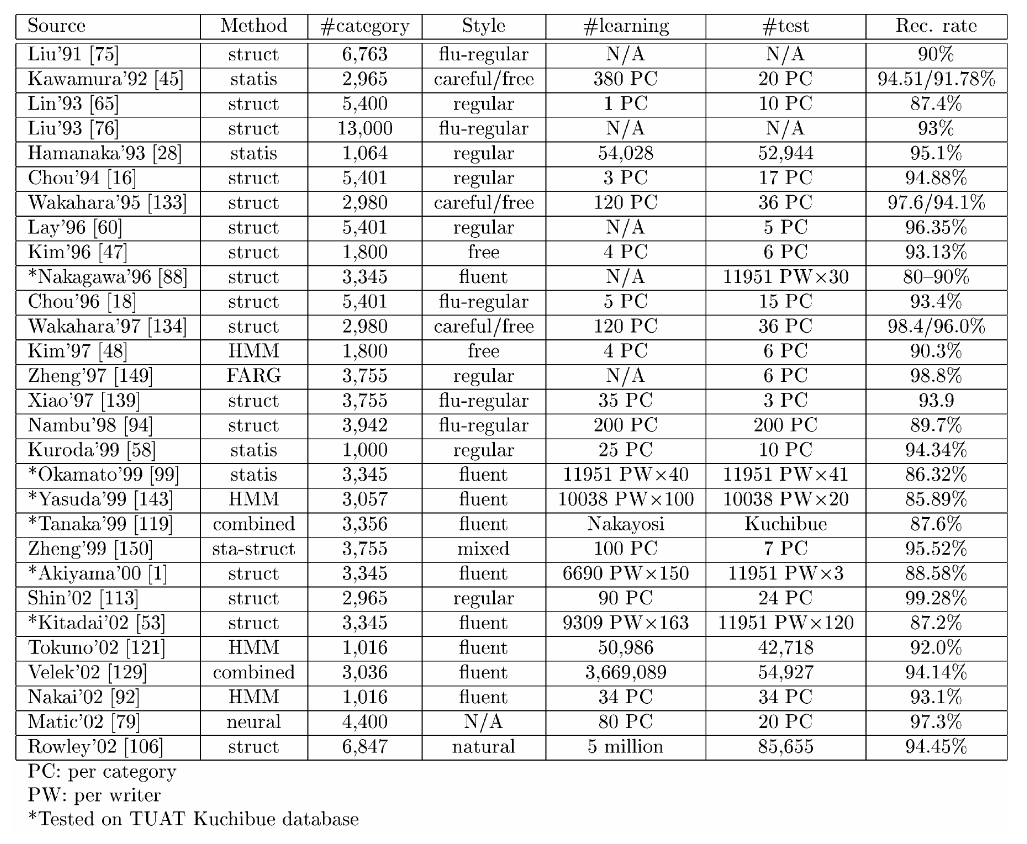
\includegraphics[scale=0.6]{images/recognitionRatesLiuJaeger.png}
    \caption{Recognition rates reported in the literature}
    \label{fig:recognitionratesreported}
  \end{center}
\end{figure}

\subsection{Development of Appropriate Evaluation Metrics}
\label{sec:eval:developmentofevalmetrics}

\subsubsection{Choice of Evaluation Subjects}
\label{sec:eval:evaluationsubjects}
It is difficult to perform an accuracy evaluation of a recognition system
that can be compared to other systems. The methods the systems use in order
to perform their recognition are diverse. There is always a trade-off between
robustness, performance and accuracy.
The prototype that is subject to this evaluation performs a different
task than most of the other recognition systems. It analyses the characters
not only for the purpose of recognition, but attempts to create feedback on
how well the input matched the character model in structural terms.
\begin{figure}[htbp]
  \begin{center}
    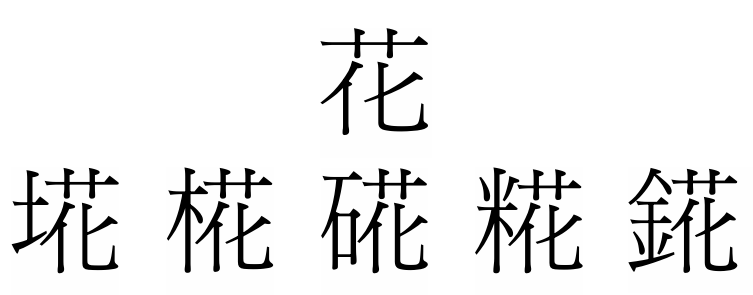
\includegraphics[scale=0.4]{images/simlarCharaters.png}
    \caption{Similar characters that can be confusing to learners: Five different Kanji share the same Radical in the \emph{tsukuri} position (on the right).}
    \label{fig:similarcharactersforuserconfusion}
  \end{center}
\end{figure}
That means concretely, the system can analyse an input with an expected result
and can perform the same for an unknown input by assuming the best match
as the expected result. The analysis yields an output that includes more
information than pure pattern matching. It rather includes structural linguistic 
information.

For example, the characters 
\cjk{埖}, \cjk{椛}, \cjk{硴}, \cjk{糀} and \cjk{錵} all share the substructure
on the right: \cjk{花}.
Figure~\ref{fig:similarcharactersforuserconfusion} shows the
substructure on top and below five characters that are using the structure.
The system analyses and distinguishes substructures. If the system is set
up to recognise an input with an expected result the output contains
a confidence value about the input quality concerning that character.
Additionally, the error recognition module returns information about the
substructures that were found in the input.
The similarity of the characters from 
figure~\ref{fig:similarcharactersforuserconfusion} is known to
the recognition system because of the identical substructures.
If the system identifies the input as a character with identical parts
with respect to the expected character the output will contain the information
as a substructure confusion error type.

This detailed analysis creates a unique requirement for evaluation. Not only
recognition accuracy must be measured and compared to other systems,
but a new evaluation for the recognition of substructures is needed.

It seems reasonable to measure the recognition accuracy in a plain 
percentage of correctly recognised characters. 
Precision and recall are the correct measurement for the recognition of 
incorrect substructures. That way, true positives, false positives, 
true negatives and false negatives can be distinguished.
Since the system can recognise pure substructures as well, it would 
be interesting to see the accuracy of a Radical recognition.

\subsubsection{Metrics Details}
\label{sec:eval:metricsdetails}

Three experiments will be conducted in order to evaluate the analytical
handwriting recognition engine. The lexicon so far is a sample lexicon that 
contains 50 characters.

\begin{itemize}
  \item \textbf{Overall recognition accuracy}
  \item \textbf{Error recognition}
  \item \textbf{Substructure recognition accuracy}
\end{itemize}

The overall recognition accuracy will be calculated as a measure of
the \(n\)-best matches for a character input. \(N\) is defined as the number
of the \(n\)-best match that will still be considered.
That is, if \(N = 1\) only the best match will be considered, if \(N = 3\)
the best three matches will be taken into account.
The overall recognition accuracy \(A_{N}\) is defined as the weighted 
percentage of correctly recognised characters when taking the \(n\)-best 
matches up to \(N\) into account. The number of samples will be called \(S\).
\(n\) is an integer between \(1\) and \(N\). If a character has a 
confidence value high enough to be the \(n\)-best match, \(\frac{1}{n}\) will
be added to the number of correctly recognised characters.
That means if a character is the best match, then \(n = 1\). 
Therefore \(\frac{1}{n} = \frac{1}{1} = 1\) will be added to the nuber of 
correct matches. If the correct character is the second best match, 
\(\frac{1}{2}\) will be added. If the character has been recognised as the 
\(n\)-best match, but \(n > N\) or the character has not been recognised at all,
nothing will be added. \(f\) is a helper function that returns a value
according to the relation between \(n\) and \(N\).
 \(A_N\) will be calculated as follows:

 \begin{quote}
 \(
f(n):=
  \begin{cases}
    \frac{1}{n} & \quad \text{if $n \leq N$}\\
    0 & \quad \text{if $n > N$}
  \end{cases}

     A_N := \frac{1}{S} \cdot \sum\limits_{i=1}^{S}{f(n)} 
 \)
 \end{quote}

 % \begin{quote}
 % \(
 %     A_N := \sqrt{(x_{i+1}-x_{i})^2+(y_{i+1}-y_{i})^2}\\
 %     l := \sum\limits_{i=1}^{N-1}{d_i} \\
 %     <x_{min} - \frac{s-w}{2},y_{min}> & \quad \text{if $s$ equals $h$}\\
 % \)
 % \end{quote}






        For the experiment concerning the overall recognition accuracy 
        two writers wrote all 50 characters as input for the system.
        The overall will be calculated as the average of the 
        The percentage of correctly recognised characters






\subsubsection{Baseline Definition}
\label{sec:eval:baselinedefinition}


% grundsaetzliches:
% evaluation soll kurz und qualitativ sein.
% plausible fakten muessen nicht unbedingt untermaurert werden.

% baseline eval vs.\ topline eval.
% technik ermoeglicht erst lernmethode, diese methode ist besser als andere methode.
% kriterium fuer qualitative eval:
% reproduzierbarkeit des experiments.

% evaluation method: counting precision and recall
% section about precision and recall - the odd numbers.
% how can that be done honest and useful?
% how can I get meaningful numbers at all?


